K reševanju sem pristopil z zapisom diferencialnih enačb, ki pogojujejo obliko vrvice. Pripravil sem funkcijo, ki iz začetnih pogojev integrira silo, kot in prostorski koordinati po brezdimenzijski ločni dolžini. Pri tem sem uporabil integrator z adaptivnim korakom (\texttt{scipy.integrate.ode}), za iskanje ničel pa vektorsko funkcijo \texttt{scipy.optimize.root}, ki mi je omogočala \emph{hkratno} iskanje končnega pogoja $x_{-1} = 0$ in $y_{-1} = y_f$. Ko sem s strelsko metodo določil začetna pogoja $F_0$ in $\alpha_0$ pri želeni spremenljivki $\beta$, sem za 200 točk na vrvi izračunal njihove pozicije in jih prikazal. Za iskanje ničel sem potreboval začetne ocene za $F_0$ in $\alpha_0$, kar sem rešil tako, da sem uporabil generator naključnega števila med 0~in~1 za začetno silo, za začetni kot pa sem generiral število med 0~in~$2\pi$. Če rutina ni našla ničle, sem generacijo začetnih približkov pognal ponovno, pri čemer sem poskušanje omejil na 100 poskusov. Kot se je izkazalo, sem le izjemoma potreboval več kot 1 poskus. Prednost takega postopka je bolj pestra in netrivialna oblika vrvi. Nekaj oblik prikazujem spodaj. Opazimo, da tudi pri nehvaležnih oblikah, ki na slikah izgledajo špičasto, integrator ne odpove in nas verno pripelje v končno točko; slika je špičasta zgolj zaradi prikaza končnega števila točk s fiksnim korakom.

\begin{center}
    \begin{minipage}{0.5\textwidth}
        \centering
    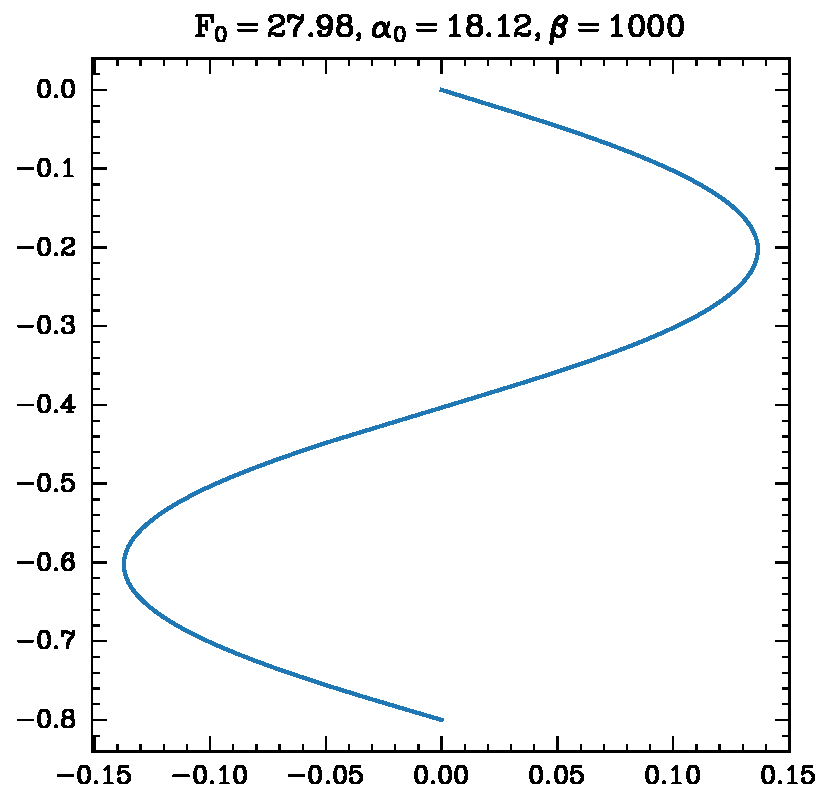
\includegraphics[width=\textwidth]{../images/2024-1-trajektorija0.pdf}
    \end{minipage}\hfill
    \begin{minipage}{0.5\textwidth}
        \centering
        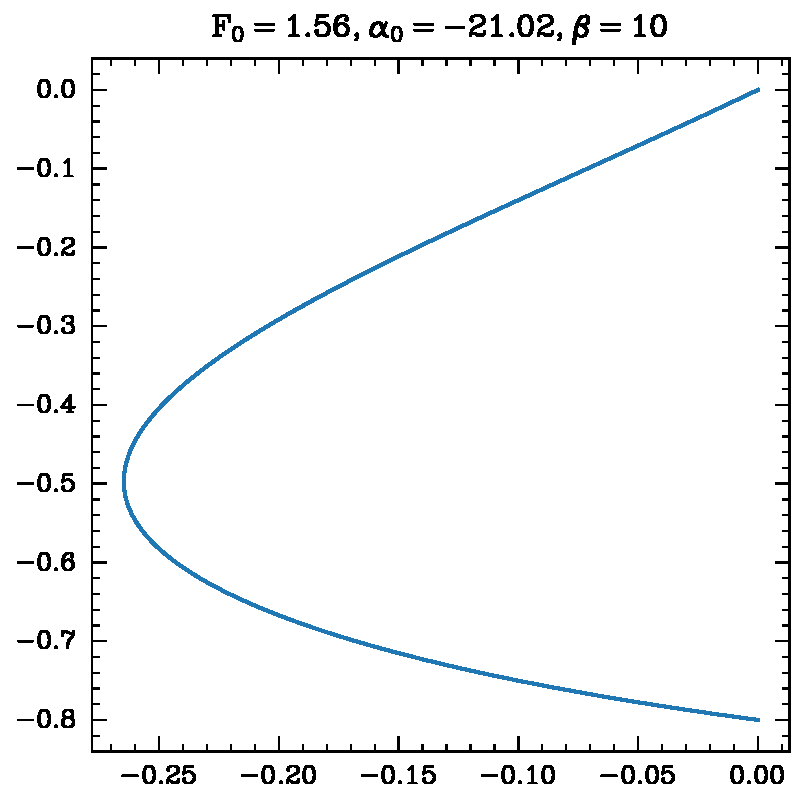
\includegraphics[width=1\textwidth]{../images/2024-1-trajektorija7.pdf}
    \end{minipage}
\end{center}
\begin{center}
    \begin{minipage}{0.5\textwidth}
        \centering
    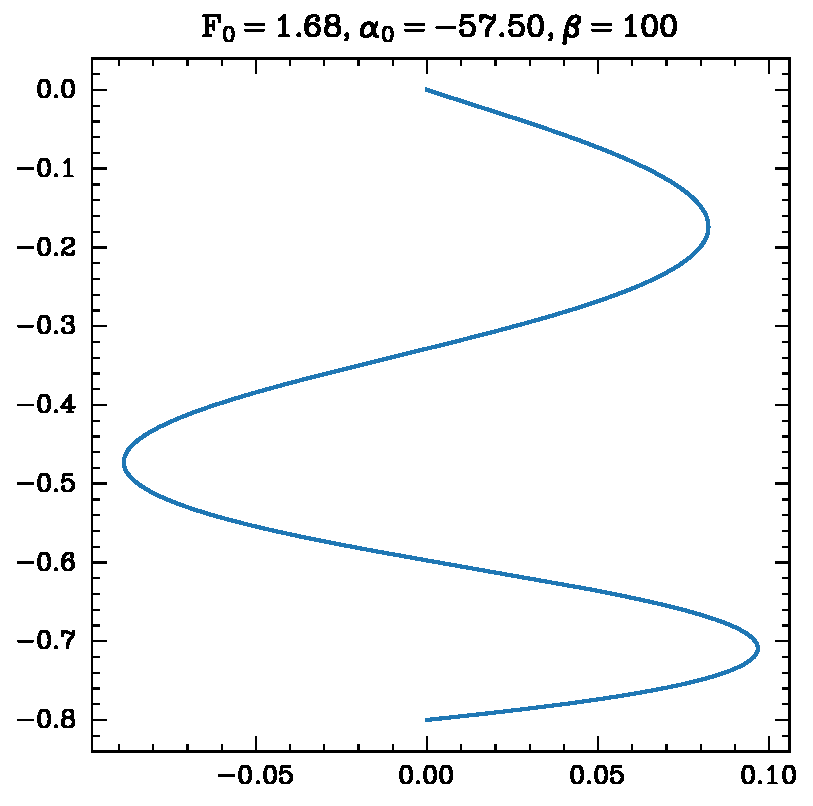
\includegraphics[width=\textwidth]{../images/2024-1-trajektorija3.pdf}
    \end{minipage}\hfill
    \begin{minipage}{0.5\textwidth}
        \centering
        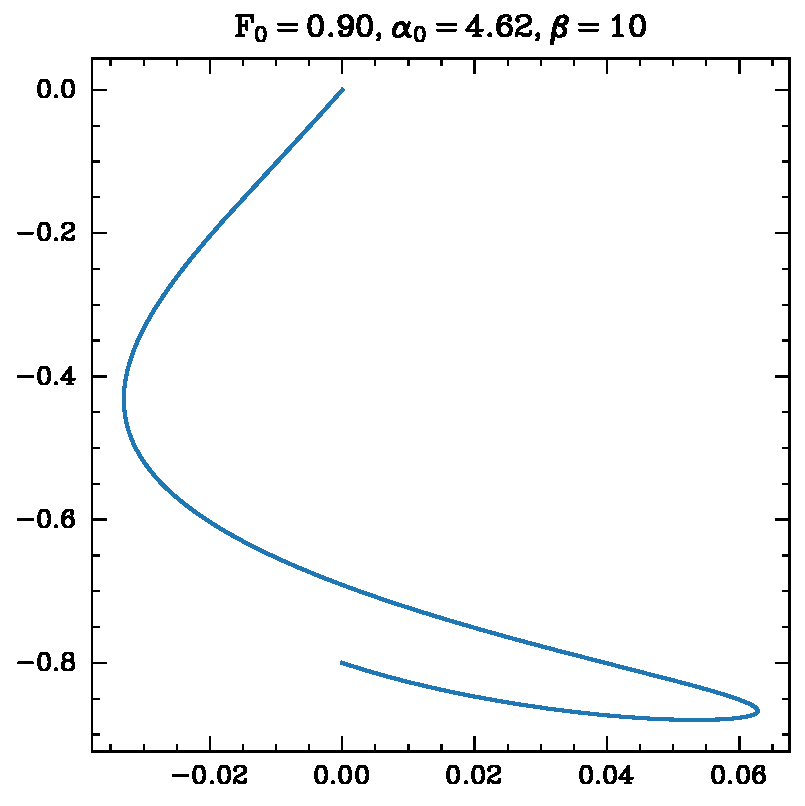
\includegraphics[width=1\textwidth]{../images/2024-1-trajektorija8.pdf}
    \end{minipage}
\end{center}
\begin{center}
    \begin{minipage}{0.5\textwidth}
        \centering
    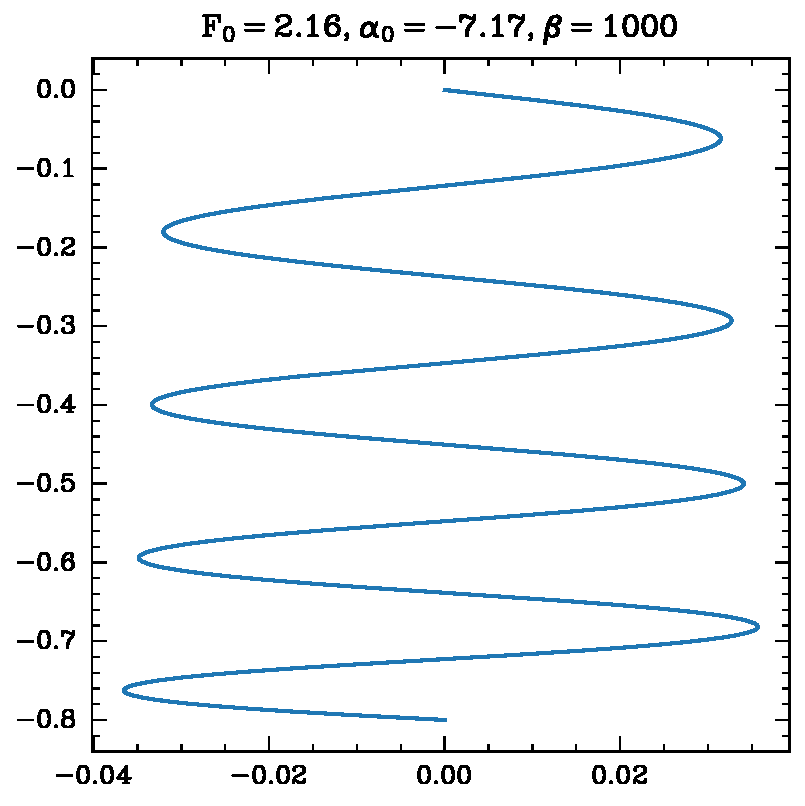
\includegraphics[width=\textwidth]{../images/2024-1-trajektorija2.pdf}
    \end{minipage}\hfill
    \begin{minipage}{0.5\textwidth}
        \centering
        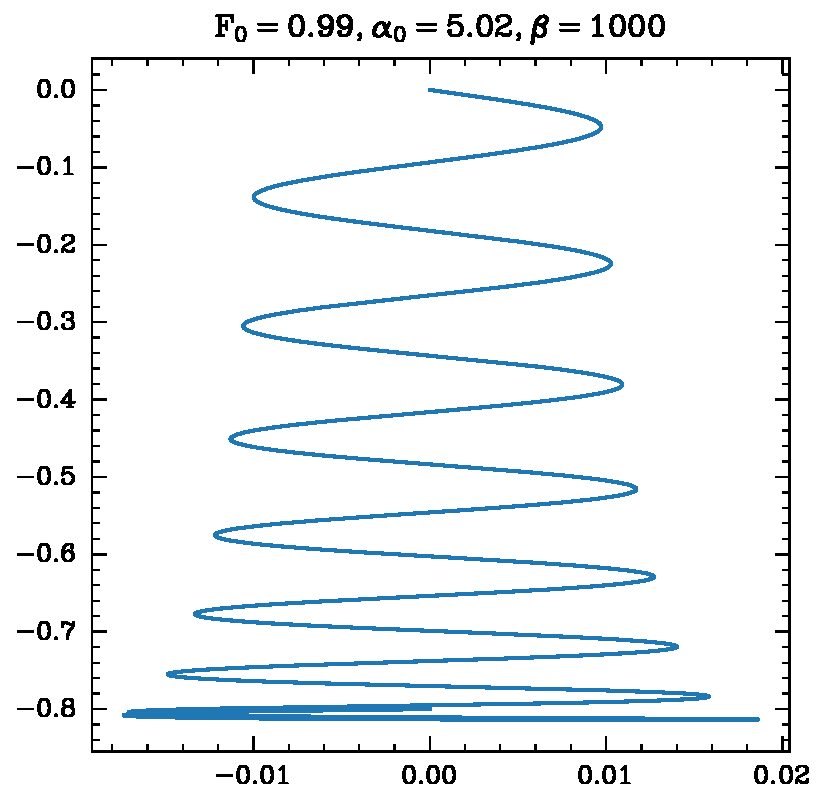
\includegraphics[width=1\textwidth]{../images/2024-1-trajektorija1.pdf}
    \end{minipage}
\end{center}


Prikazane oblike so skalirane v vodoravni smeri. Hitro opazimo, da lahko pri isti vrednostih $\beta$ in $y_f$ najdemo več kvalitativno različnih oblik vrvi. Da bi korektno raziskal oblike vrvi, sem sestavil funkcije, ki preštejejo število sprememb predznaka, določijo maksimalen absolutni odmik od osi $y$ in maksimalno globino vrvi. Ker so ponekod oblike degenerirane, sem za različne $\beta$ in $y_f$ najprej poiskal rešitve in jih opisal s funkcijami, vrednosti funkcij pa prikazal na 3D grafih.
\begin{center}
     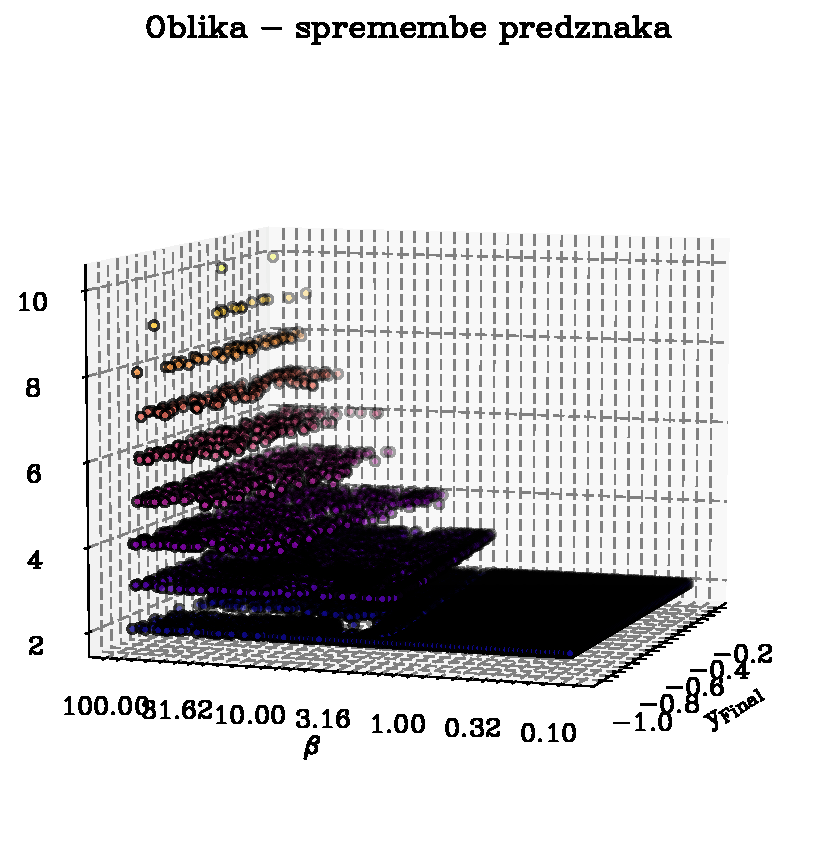
\includegraphics[width=0.9\textwidth]{../images/2024-1-fazni_portret_spremembe_opredznaka.pdf}
\end{center}
Pri spremembi predznaka je opazen globalen minimum pri vrednosti 2, kar lahko pojasnimo z definicijo funkcije
\[ \mathrm{Signum}\; (x) = \begin{cases}
-1 &\mbox{če } x < 0, \\
\phantom{-}0  & \mbox{če } x = 0, \\
\phantom{-}1  & \mbox{če } x > 1.
\end{cases}\]
Ker integracijo vedno začnemo in končamo  pri $x = 0$, nam vsaka oblika prinese najmanj 2 spremembi predznaka, razen v primeru, da celotna trajektorija leži na $x=0$. Opazimo, da z naraščanjem kotne frekvence najdemo vedno bolj pestre rešitve, vpliv končnega pritrdišča točke pa na pestrost ne vpliva dosti. Pri visokih $\beta$ je opaziti polje, kjer v nobenem primeru ne najdemo rešitev, ki bi dvakrat spremenile predznak.


Za maksimalno globino t.j. minimalno vrednost $y$ koordinate velja, da je pri \emph{razpeti} neraztegljivi vrvi (torej ko je $y_f=-1$) enaka ne glede na vrednost parametra $\beta$. Tedaj je vrv popolnoma raztegnjena, vsaka trajektorija je zgolj zveznica med izhodiščem in točko $(0,y_f) = (0, -1)$. Če spodnje pritrdišče variiramo, opazimo dve ravnini rešitev. V ravnini ($\beta, y_\mathrm{min}$) dobimo zanimive vzorce, ki pa se pojavijo šele, ko $\beta$ preseže kritično vrednost:
\begin{center}
     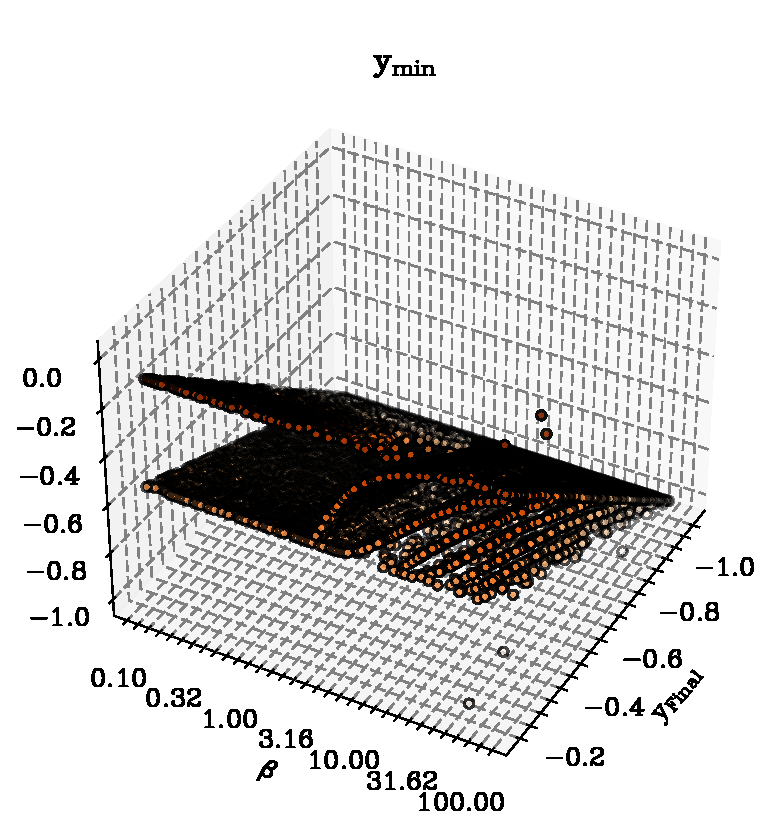
\includegraphics[width=0.9\textwidth]{../images/2024-1-fazni_portret_ymin.pdf}
\end{center}

Za maksimalen odmik od navpične osi velja podobno: pri nizkih $\beta$ se ne dogaja kaj dosti zanimivega, nad neko kritično vrednostjo pa lahko najdemo več ploskev rešitev, ki so presenetljivo zvezne in distinktno ločene med seboj. Tudi tu vpliv spodnjega pritrdišča ni močen, razen pri distalnem robu slike, ko $y_{Final} \rightarrow -1 $. Tu je vrv napeta, in deviacija od navpične osi ni mogoča.
\begin{center}
     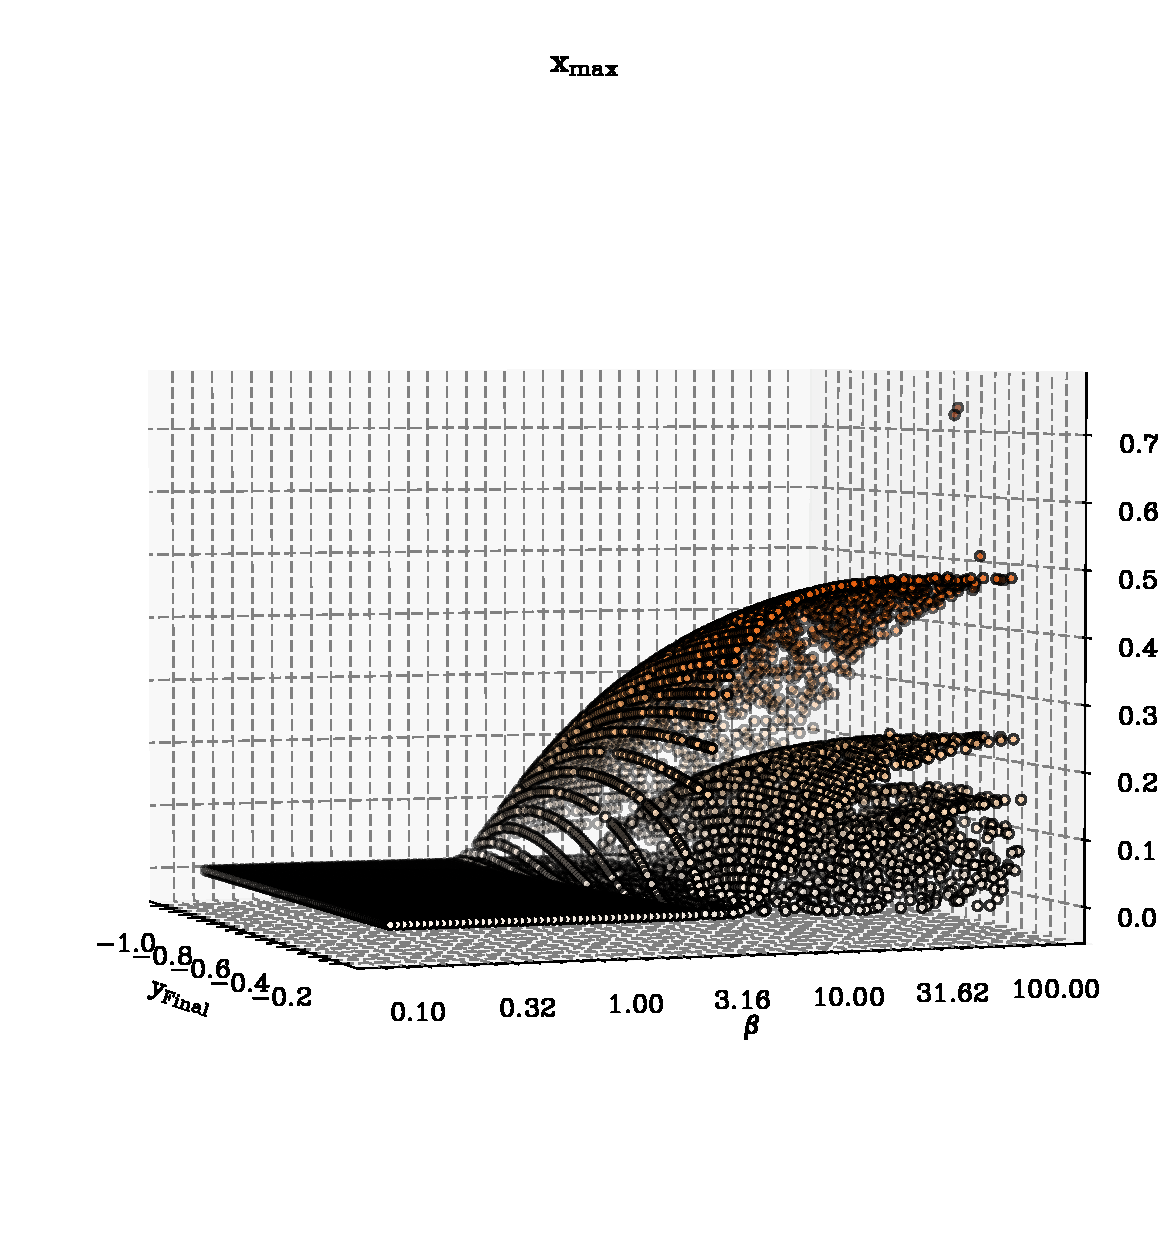
\includegraphics[width=0.9\textwidth]{../images/2024-1-fazni_portret_xmax.pdf}
\end{center}

Preverim lahko še obnašanje v limitah $\omega \rightarrow \infty$ in $\omega \rightarrow 0$. Za slednji primer lahko uporabim doslej uporabljeni cevovod, za velike vrednosti $\omega$ pa moram popraviti žrebanje začetnih približkov tako, da se sila v pritrdišču žreba iz bistveno večjega intervala, kar mi omogoča najti najbolj razpete vrvi. Pri $\beta=0$ opazimo, da vrv ne konča več v $x = 0$, ampak $2\mathrm{e} {-10}$ stran, ker za ta limitni primer optimizator odpove.

\begin{center}
    \begin{minipage}{0.5\textwidth}
        \centering
    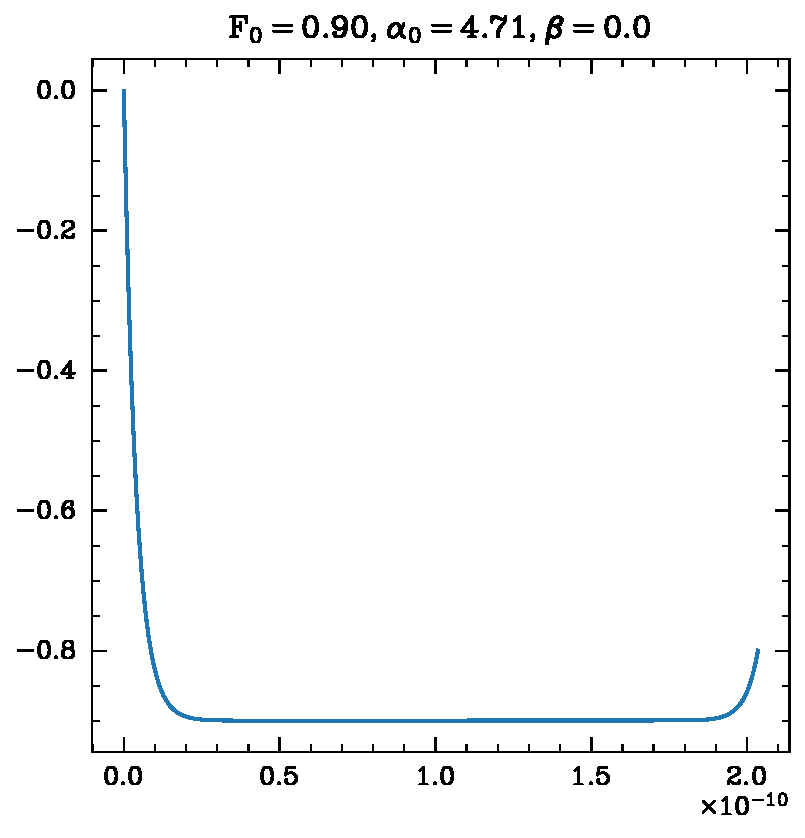
\includegraphics[width=\textwidth]{../images/2024-1-trajektorija_limit_beta0.pdf}
    \end{minipage}\hfill
    \begin{minipage}{0.5\textwidth}
        \centering
        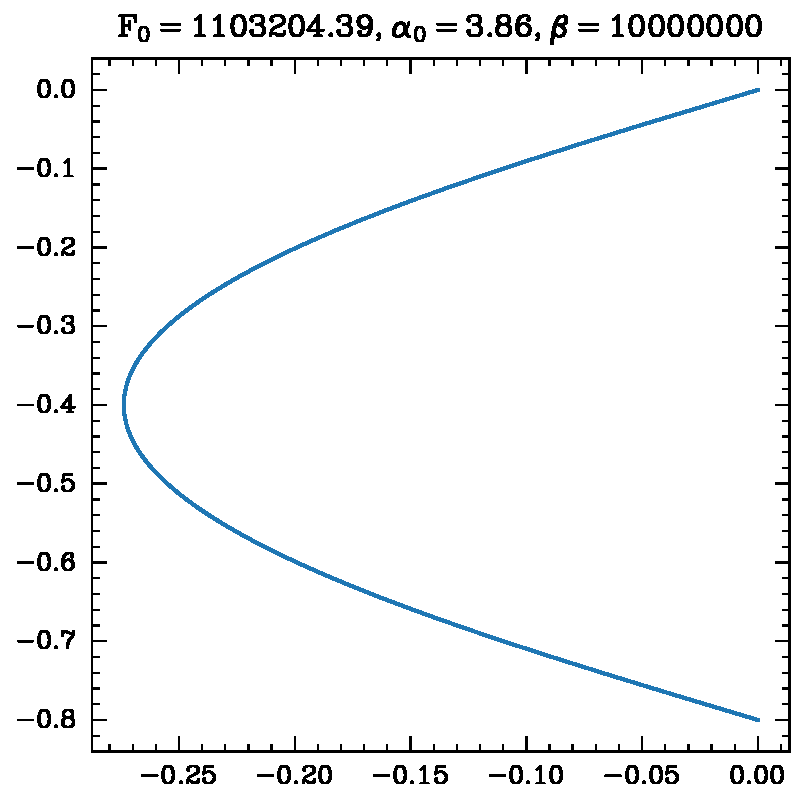
\includegraphics[width=1\textwidth]{../images/2024-1-trajektorija_limit_betainf.pdf}
    \end{minipage}
\end{center}

Preveril sem tudi ohranitev dolžine. Pri diskretizaciji z 2000 elementi se dolžina ohrani na $0.5\mathrm{e}{-4}$, pri določenih vrednostih $\beta$ še dosti bolj, opazen pa je tudi trend pri nizkih vrednostih $\beta$, kjer konsistentno in monotono 'izgubljamo' dolžino med integracijo.
\begin{center}
    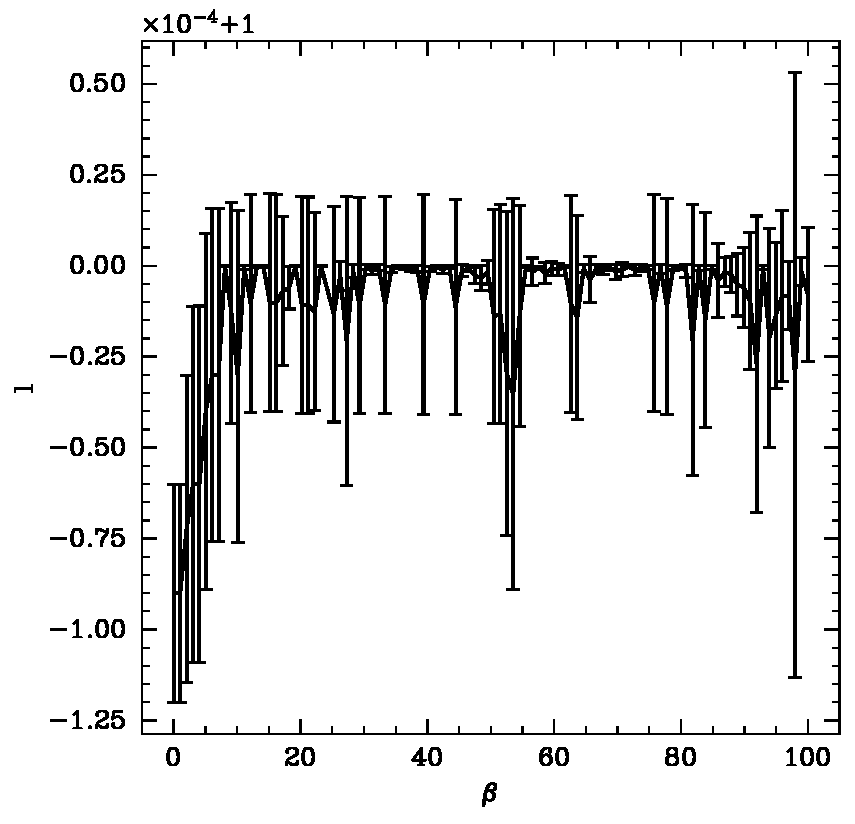
\includegraphics[width=0.7\textwidth]{../images/2024-1-ohranitev_dolzine.pdf}
\end{center}
